%!TEX root = lec05_query_processing.tex


\begin{frame}

Recall that indexes as \emph{associative access methods} that allow the DBMS to quickly find tuples based on the values of their attributes.

B+ tree indexes, hash tables and hash sets can be used to implement many query plan operators: selections, joins (and their variants), all set operators, duplicate elimination, and grouping.

The next slides give some examples of the use of indexes.

We start by looking at \textbf{base indexes}, or indexes created by the database administrator, and discuss briefly the idea of on-the-fly indexing, which is to create an index with the result of a sub-query to be used once.

\end{frame}

\begin{frame}[fragile]

\vskip1em
The table below indicates, generally, which kinds of predicates can be improved by the use of \textbf{indexes}.

\vskip1.5em

\begin{center}
\begin{tabular}{l||c|c|c||c|c}
\hline
& $a_i = v$ & $a_i \geq v$ & $a_i$ \texttt{\footnotesize IN ()} & $a_i \neq v$ &  $a_i$ \texttt{\footnotesize NOT IN ()}\\
\hline\hline
B+ tree & \cmark & \cmark$^\dagger$ & \cmark & \xmark$^\ddagger$ & \cmark\\
Hash table & \cmark & \xmark & \cmark & \xmark$^\ddagger$ & \cmark\\
\hline
\end{tabular}
\end{center}

\vskip1em

\footnotesize

$^\dagger$ If the B+tree is a secondary index and the selectivity of the predicate is high, a table scan might be better.

$^\ddagger$ These predicates often \alert{have very high selectivity}, so the table scan is \alert{almost always better}.

\normalsize
\end{frame}

%
% -----------------------------------------------------------------------
%

\newsavebox{\PickingIndexesExample}
\begin{lrbox}{\PickingIndexesExample}
\begin{lstlisting}[style=SQL]
SELECT director
FROM Movie
WHERE title='Ghostbusters' AND year=1984
\end{lstlisting}
\end{lrbox}

\begin{frame}[fragile]{How are Indexes Chosen?}

A predicate \alert{\lstinline[mathescape]!$a_i\ $<op>$\ v$!} in the \lstinline[style=SQL]{WHERE} clause can be answered using an index only if \alert{$a_i$ is a prefix of the index key}.

\vskip1em

\textbf{Example:}\qquad \framebox{\scalebox{0.8}{\usebox\PickingIndexesExample}}

\vskip1em

\begin{columns}[onlytextwidth]
\begin{column}{0.45\textwidth}
\begin{block}{Useful Indexes}
\lstinline[style=SQL]{Movie(title)}, ~~~~ \lstinline[style=SQL]{Movie(year)},\\
\lstinline[style=SQL]{Movie(title,imdb)}, ... 
\end{block}
\end{column}
\begin{column}{0.45\textwidth}
\begin{block}{Not Useful}
\lstinline[style=SQL]{Movie(imdb,title)}, \\
\lstinline[style=SQL]{Movie(director)} ... 
\end{block}
\end{column}
\end{columns}

\vskip1em
If multiple useful indexes exist, the DBMS picks the one with lowest estimated cost, which depends on the selectivity of the predicate!
\end{frame}


%
% -----------------------------------------------------------------------
%
\begin{frame}[fragile]

\begin{center}
\small
\begin{tabular}{r|l}
$T(\text{Movie}) = 100,000$ & $V(\text{Movie}, \text{title}) = 95,000$ \\
$S(\text{Movie}) = 92$ & $V(\text{Movie}, \text{year}) = 32$ \\
$B(\text{Movie}) = 2,000$ & $V(\text{Movie}, \text{imdb}) = 50$ \\
 & $V(\text{Movie}, \text{director}) = 25,000$ \\
\end{tabular}
\normalsize
\end{center}

\vskip2em

Suppose we have the following B+ tree indexes with 100 pointers/node.

\vskip1em

\begin{quote}
\lstinline[style=SQL]{> CREATE INDEX IDX1 ON Movie(Title);}
\lstinline[style=SQL]{> CREATE INDEX IDX2 ON Movie(Title,Year);}
\lstinline[style=SQL]{> CREATE INDEX IDX3 ON Movie(Year);}
\end{quote}

In all cases, 3 levels are enough to index all keys.

\end{frame}


\begin{frame}[fragile]

How many blocks (at the leaf level) of each index will have tuples matching the query?

\small
\[T(\sigma_{\texttt{title='Ghostbusters'}}(\texttt{Movie})) = \ceil*{\frac{100,000}{95,000}}=2\]
\[T(\sigma_{\texttt{year=1984}}(\texttt{Movie})) = \ceil*{\frac{100,000}{32}}=3,125\]
\normalsize

\vskip1em

\begin{block}{\alert{We can thus expect to find:}}
 - all movies with that title in a single \textbf{leaf} block of \lstinline[style=SQL]{IDX1}\\
 - all movies from 1984 in 32 \textbf{leaf} blocks of \lstinline[style=SQL]{IDX3}\\
 - all movies with that title/year in a single \textbf{leaf} block of \lstinline[style=SQL]{IDX2}
\end{block}
\end{frame}

%
% -----------------------------------------------------------------------
%
\begin{frame}[fragile]

\begin{center}
\framebox{\scalebox{0.8}{\usebox\PickingIndexesExample}}
\end{center}

\vskip2em

\begin{columns}
\begin{column}{0.125\textwidth}
\begin{tikzpicture}[semithick,align=center,node distance=0.75cm,every node/.style={inner sep=1,outer sep=1,font=\footnotesize}]
\node (0) at (0,0) {} ; %empty node with ``answer''
\node (1) [below of= 0] {$\pi_{\texttt{director}}$};
\node (2) [below of= 1] {$\sigma_{\substack{\texttt{title='Ghostbusters'}\\\wedge\, \texttt{year=1984}}}$};
\node (3) [below of= 2] {\lstinline[style=SQL]{scan(Movie)}};
\path[->]
    (3) edge (2)
    (2) edge (1)
    (1) edge (0);
\end{tikzpicture}
\end{column}
\begin{column}{0.5\textwidth}
\begin{center}
\begin{tikzpicture}[semithick,align=center,node distance=0.8cm,every node/.style={inner sep=1,outer sep=1,font=\footnotesize}]
\node (0) at (0,0) {} ; %empty node with ``answer''
\node (1) [below of= 0] {$\pi_{\texttt{director}}$};
\node (2) [below of= 1] {$\sigma_{\texttt{year=1984}}$};
\node (3) [below of= 2] {\lstinline[style=SQL]{pointer_lookup}};
\node (4) [below of= 3] {\lstinline[style=SQL]{search(IDX1, =, "Ghostbusters")}};
\path[->]
    (4) edge (3)
    (3) edge (2)
    (2) edge (1)
    (1) edge (0);

\pause
\node (5) [node distance=2.5cm,left of=2,color=blue] {\begin{minipage}{2.15cm}\baselineskip=0.75\baselineskip \centering
follow the pointer to get the entire tuple 
\end{minipage}};
\draw [color=blue,->] (5) -- (3);
\end{tikzpicture}
\end{center}
\end{column}
\end{columns}

\vskip1em

\begin{block}{\alert{Estimated I/O costs:}}
 - left plan: 2,000 blocks\\
 - right plan: 3 \textcolor{blue}{+ 2} = \alert{5} blocks\footnotemark
\end{block}

\footnotetext{3 I/Os on the index (root to leaf path) + 2 lookups on the table.}

\end{frame}

%
% -----------------------------------------------------------------------
%

\begin{frame}{Cost recap}

The cost of retrieving tuples from a table $R$ satisfying a predicate $p$ using a a \alert{B+ Tree} with $|I|$ blocks at the \emph{leaf level} is the sum of:

\begin{enumerate}[(1),noitemsep]
\item Number of inner blocks in the path from root to the first index leaf (usually 2 or 3).
\item Number of blocks of the index that will be read: \(\ceil*{s(p) \cdot |I|}\). 
\item Number of pointer lookups: \(T(\sigma_p (R))\) (unless this is a primary index and the table is sorted as the index).
\end{enumerate}

\vskip1em

With a \alert{hash table}, the estimated cost is \(T(\sigma_p (R)) \cdot 2\): one read in the hash table and another for the pointer traversal to the table.

\end{frame}


%
% -----------------------------------------------------------------------
%
\begin{frame}[fragile]{Covering Index}

The \alert{\lstinline[style=SQL]{pointer_lookup}} operator pulls a pointer to a tuple in \lstinline[style=SQL]{Movie} returned by the index search operator and goes to the block of file of the \lstinline[style=SQL]{Movie} table that contains the respective tuple and fetches it.

This operator is needed because the query uses attributes of \lstinline[style=SQL]{Movie} that are not present in the index record (\lstinline[style=SQL]{year} and \lstinline[style=SQL]{director}).

\vskip1em

\begin{columns}[onlytextwidth]
\begin{column}{0.45\textwidth}
An index with all attributes from the table used in a query is called a \alert{covering index}.
\end{column}

\begin{column}{0.5\textwidth}
\begin{lstlisting}[style=SQL]
SELECT year
FROM Movie
WHERE title='Ghostbusters'
\end{lstlisting}
\end{column}
\end{columns}

\lstinline[style=SQL]{IDX2} is a covering index for the query above.

\end{frame}

%
% -----------------------------------------------------------------------
%
\begin{frame}[fragile]{Index-Based Joins}

Depending on whether the index is primary or not, and on the selectivity of a join predicate, the DBMS might use a base index to speed up a nested-loop join:

% \vskip1em

\begin{columns}[onlytextwidth]
\begin{column}{0.35\textwidth}
\begin{lstlisting}[style=SQL,basicstyle=\scriptsize\ttfamily]
SELECT role, imdb
FROM Movie 
  JOIN Cast 
WHERE actor='Bill Murray';
\end{lstlisting}
\end{column}
\begin{column}{0.6\textwidth}
\begin{center}
\vspace*{-2em}
\scalebox{0.85}{
    \begin{tikzpicture}[semithick,align=center,node distance=0.875cm,every node/.style={inner sep=1,outer sep=1,font=\footnotesize}]
\node (0) at (0,0) {} ; %empty node with ``answer''
\node (1) [below of= 0] {$\pi_{\texttt{role,imdb}}$};

\node (2) [below of= 1] {$\Join$};
\node (3) [below right= of 2] {\lstinline[style=SQL]{pointer_lookup}} ;
\node (4) [below left= of 2] {$\sigma_{\texttt{actor='Bill Murray'}}$};
\node (5) [below of= 3] {\lstinline[style=SQL,mathescape]!search(IDX2, =, (t.title, t.year))!};
\node (6) [below of =4] {\lstinline[style=SQL]{scan(Cast)}};

\draw[->,color=accent,thick,densely dotted] (2) to[out=270,in=135] (5.north west);

\path[commutative diagrams/.cd, every arrow, every label]
    (6) edge (4)
    (4) edge node {$t$} (2) 
    (5) edge (3)
    (3) edge (2)
    (2) edge (1)
    (1) edge (0);
\end{tikzpicture}
}
\end{center}
\end{column}
\end{columns}

\vskip1em

The I/O cost is bound by $s(\text{Cast},\text{actor='Bill Murray'})$.

Of course, if there was an index on \lstinline[style=SQL]{Cast(actor)}, it could also be used instead of the table scan in the example above.

\end{frame}

\begin{frame}[fragile]{On the Fly Indexing}

\vskip2em

\begin{columns}[onlytextwidth]
\begin{column}{0.45\textwidth}

The DBMS might create an index/hash table/hash set with the results of a sub-query to speed up a join.

\vskip1em

\begin{lstlisting}[style=SQL,basicstyle=\scriptsize\ttfamily]
SELECT actor, role
FROM Cast
WHERE (title,year) IN (
    SELECT film, year
    FROM Guide
    WHERE theater='Garneau');
\end{lstlisting}
\end{column}
\begin{column}{0.5\textwidth}
\begin{center}
\vspace*{-2em}
\scalebox{0.85}{
    \begin{tikzpicture}[semithick,align=center,node distance=0.875cm,every node/.style={inner sep=1,outer sep=1,font=\footnotesize}]
\node (0) at (0,0) {} ; %empty node with ``answer''
\node (1) [below of= 0] {$\pi_{\texttt{actor,role}}$};
\node (2) [below of= 1] {\alert{$\ltimes$}};
\node (3) [below left= of 2] {\lstinline[style=SQL]{scan(Cast)}}; 
\node (4) [below right= of 2] {\lstinline[style=SQL]{create_hash_set()}} ;
\node (5) [below of= 4] {$\pi_{\texttt{film,year}}$};
\node (6) [below of= 5] {$\sigma_{\texttt{theater}=\text{``Garneau''}}$};
\node (7) [below of= 6] {\lstinline[style=SQL]{scan(Guide)}};

\path[->]
    (7) edge (6)
    (6) edge (5)
    (5) edge (4)
    (4) edge (2) 
    (3) edge (2)
    (2) edge (1)
    (1) edge (0);
\end{tikzpicture}
}
\end{center}
\end{column}
\end{columns}

\vskip1em

Recall the \textbf{semijoin} \alert{$R \ltimes S$} returns tuples from $R$ that match a tuple in $S$ with respect to the join attributes (\lstinline[style=SQL]{title,year}).

\end{frame}


\begin{frame}[fragile]{Answering Complex Predicates with Secondary Indexes}

Primary indexes allow the fastest access to tuples in the corresponding table because \alert{the tuples in the table file are sorted in the same way as the keys in the index}.\\
 - these indexes are sometimes called \textbf{clustered indexes}

\vskip1em

The problem is there can be only one primary index per table.

\vskip1em

A way to bring some of the benefits of primary to secondary indexes is to \textbf{cluster tuple identifiers} based on search key in an a ``bucket file'' and have a primary index over that file.

\end{frame}


%
% Key-pointer measurements
%
\newlength{\indexKeyBoxWidth}
\setlength{\indexKeyBoxWidth}{\dimexpr 2em\relax}

\newlength{\pointerBoxWidth}
\setlength{\pointerBoxWidth}{\dimexpr 2.5em\relax}

%
% Tuple measurements
%
\newlength{\tupleHeight}
\setlength{\tupleHeight}{\dimexpr 1.1em\relax}

\newlength{\dummyTupleGreyBoxWidth}
\setlength{\dummyTupleGreyBoxWidth}{\dimexpr 5em\relax}

%
% Data Block measurements
%

\newlength{\tupleWidth}
\setlength{\tupleWidth}{\dimexpr(\indexKeyBoxWidth+\dummyTupleGreyBoxWidth)\relax}

\newlength{\dataBlockWidth}
\setlength{\dataBlockWidth}{\dimexpr(\tupleWidth+1pt)\relax}

\def\tuplesPerDataBlock{2}

\newlength{\dataBlockHeight}
\setlength{\dataBlockHeight}{\dimexpr1pt+(\tupleHeight+0.5pt)*\the\numexpr\tuplesPerDataBlock\relax}

%
% Index block measurements
%
\newlength{\indexBlockWidth}
\setlength{\indexBlockWidth}{\dimexpr(\indexKeyBoxWidth+\pointerBoxWidth+1pt)\relax}

\def\keyPointerPairsPerIndexBlock{4}

\newlength{\indexBlockHeight}
\setlength{\indexBlockHeight}{\dimexpr1pt+(\tupleHeight+0.5pt)*\the\numexpr\keyPointerPairsPerIndexBlock\relax}

\newlength{\indexBlockPointerOffset}
\setlength{\indexBlockPointerOffset}{\dimexpr(\indexBlockHeight-1em-1pt)\relax}


\tikzset{ % same as tuple, except for the anchor part
	indexKeyBox/.style={
		draw,rectangle,minimum width=\indexKeyBoxWidth,minimum height=\tupleHeight,inner sep=0,outer sep=0,font=\footnotesize
	}
}

\tikzset{
	tupleGrayBox/.style={
		draw, rectangle, minimum width=\dummyTupleGreyBoxWidth,minimum height=\tupleHeight,outer sep=0,fill=tupleBoxColor
	}
}

% #1 --> block id
% #2,#3 --> data block id and order inside block
% #4 --> key
\def\tuple#1#2#3#4{
  \node ({#1}) at ([xshift=1pt,yshift=\dimexpr -1pt-(\tupleHeight+0.5pt)*#3]{#2}.north west) [anchor=north west,indexKeyBox] {{#4}};
  \node [right = -0.5pt of {#1}] [tupleGrayBox] {};
}


% #1 --> block id
% #2,#3 --> data block id and order inside block
% #4 --> key
\def\tupleFromBox#1#2#3#4{
  \node ({#1}) at ([xshift=1pt,yshift=\dimexpr -1pt-(\tupleHeight+0.5pt)*#3]{#2}.north west) [anchor=north west,indexKeyBox] {{#4}};
}


% --------------------------------- index key-pointer tuples

\tikzset{
	keyPointerValue/.style={
		anchor=north west,
		draw,rectangle,minimum width=\indexKeyBoxWidth,minimum height=\tupleHeight,inner sep=0,outer sep=0,font=\footnotesize
	}
}

\tikzset{ 
	keyPointerPointerBox/.style={
		draw, rectangle, minimum width=\pointerBoxWidth,minimum height=\tupleHeight,outer sep=0,fill=snow
	}
}


% #1     --> id of key-pointer (i.e., the node with the value)
% #2, #3 --> id of indexBlock and ordinal within block
% #4     --> value in the attribute of the tuple
\def\keyPointer#1#2#3#4{
  \node ({#1}) at ([xshift=1pt,yshift=\dimexpr -1pt-(\tupleHeight+0.5pt)*#3]{#2}.north west) [anchor=north west,indexKeyBox] {{#4}};
  \node [right = -0.5pt of {#1}] [keyPointerPointerBox] {};
}


% --------------------------------- blocks of the data file

\tikzset{
	dataBlockBox/.style={
		xshift=-0.1em,yshift=0.1em,anchor=north west,draw,rectangle,minimum width=\dataBlockWidth,minimum height=\dataBlockHeight
	}
}

\tikzset{
	dataBlockPointerBox/.style={
		yshift=0.125pt,
		outer sep=0,anchor=south west, draw, rectangle, 
		minimum width=1em, minimum height=1em,fill=snow
	}
}

% #1     --> block id
% #2, #3 --> block top-left coordinates
\def\dataBlock#1#2#3{
	\node ({#1}) at ({#2},{#3}) [dataBlockBox] {};
	\node at ({#1}.south east) [dataBlockPointerBox] {};
}

% #1     --> block id
% #2     --> id of block ``below'' #1
\def\linkDataBlocks#1#2{
	\draw [*->,>=stealth'] ([xshift=5pt,yshift=7pt]{#1}.south east) to[out=270,in=90] ([xshift=-10pt]#2.north east);
}

% --------------------------------- blocks of the index file


\tikzset{
	indexBlockBox/.style={
		xshift=-0.1em,yshift=0.1em,anchor=north west,draw,rectangle,minimum width=\indexBlockWidth,minimum height=\indexBlockHeight
	}
}

\tikzset{
	indexBlockPointerBox/.style={
		xshift=0.375pt,
		anchor=south east, draw, rectangle, minimum width=1em, minimum height=1em,fill=snow
	}
}

% #1     --> block id
% #2, #3 --> block top-left coordinates
% #4     --> id of the first key-pointer inside the block
% #5     --> value of the first key
\def\indexBlock#1#2#3{
	\node ({#1}) at ({#2},{#3}) [indexBlockBox] {};
	\node at ({#1}.south west) [indexBlockPointerBox] {};
}

% #1     --> block id
% #2     --> id of block ``below'' #1
\def\linkIndexBlocks#1#2{
	\draw [*->,>=stealth'] ([xshift=-5pt,yshift=7pt]{#1}.south west) to[out=270,in=90] ([xshift=10pt]#2.north west);
}

% #1 --> key-pointer id
% #2 --> tuple id
\def\KPtoTuple#1#2{
	\draw [*->,>=stealth'] ([xshift=30pt,yshift=0em]{#1}.west) to[out=0,in=180] (#2.west);
}




%%%%% MACROS FOR SPARSE INDEX WITH POINTERS TO BLOCKS

\tikzset{ 
	sparseKeyPointerPointerBox/.style={
		draw, rectangle, minimum width=1.1em,minimum height=\tupleHeight, fill=snow
	}
}

% draws two rectangles, one with an attribute value, the other with the pointer
%
% #1     --> id of key-pointer (i.e., the node with the value)
% #2, #3 --> coordinages of top-left corner of node with tuple value
% #4     --> value in the attribute of the tuple
\def\sparseKeyPointer#1#2#3#4{
  \node ({#1}) at ({#2},{#3}) [keyPointerValue] {\tiny{#4}} ;
  \node [right = -0.5pt of {#1}] [sparseKeyPointerPointerBox] {};
}

\tikzset{
	sparseIndexBlockBox/.style={
		xshift=-0.1em,yshift=0.1em,anchor=north west,draw,rectangle,minimum width=3.3em,minimum height=4.6em
	}
}

% #1     --> block id
% #2, #3 --> block top-left coordinates
% #4     --> id of the first key-pointer inside the block
% #5     --> value of the first key
\def\sparseIndexBlock#1#2#3#4#5{
	\node ({#1}) at ({#2},{#3}) [sparseIndexBlockBox] {};
	\node at ({#2},{#3}) [indexBlockPointerBox] {};
	\sparseKeyPointer{{#4}}{{#2}}{{#3}}{{#5}};
}

% #1     --> block id
% #2     --> id of block ``above'' this one
% #3, #4 --> coordinates of this block
% #5     --> id of the first tuple inside the block
% #6     --> value of the first tuple
\def\sparseIndexBlockBelow#1#2#3#4#5#6{
	\node ({#1}) at ({#3},{#4}) [sparseIndexBlockBox] {};
	\node at ({#3},{#4}) [indexBlockPointerBox] {};
	\sparseKeyPointer{{#5}}{{#3}}{{#4}}{{#6}};
	\draw [*->,>=stealth'] ([xshift=-5pt,yshift=7pt]{#2}.south west) to[out=270,in=90] ([xshift=10pt]#1.north west);
}

% #1 --> key-pointer id
% #2 --> tuple id
\def\sparseKPtoTuple#1#2{
	\draw [*->,>=stealth'] ([xshift=22.5pt,yshift=0em]{#1}.west) to[out=0,in=180] (#2.west);
}



%================================ illustration of multilevel indexes

\def\denseIndexMultilevel#1#2#3#4{
    \node ({#1}) at ({#2},{#3}) [font=\footnotesize,draw,fill=accent!25,rectangle,minimum width=2.5em,minimum height=1em] {{#4}};
    \node (t) [below = 1em of {#1}] [rectangle,minimum width=2.5em] {};
    \draw [->,>=stealth'] ({#1}) -- (t);
    \draw [->,>=stealth'] ([xshift=-2pt]{#1}.south) -- ([xshift=-6pt]t.north);
    \draw [->,>=stealth'] ([xshift=2pt]{#1}.south) -- ([xshift=6pt]t.north);
    \draw [->,>=stealth'] ([xshift=-6pt]{#1}.south) -- (t.north west);
    \draw [->,>=stealth'] ([xshift=6pt]{#1}.south) -- (t.north east);
}

\def\denseIndexMultilevelAfter#1#2#3{
    \node ({#1}) [right of= {#2}] [font=\footnotesize,draw,fill=accent!25,rectangle,minimum width=2.5em,minimum height=1em] {{#3}};
        \node (t) [below = 1em of {#1}] [rectangle,minimum width=2.5em] {};
    \draw [->,>=stealth'] ({#1}) -- (t);
    \draw [->,>=stealth'] ([xshift=-2pt]{#1}.south) -- ([xshift=-6pt]t.north);
    \draw [->,>=stealth'] ([xshift=2pt]{#1}.south) -- ([xshift=6pt]t.north);
    \draw [->,>=stealth'] ([xshift=-6pt]{#1}.south) -- (t.north west);
    \draw [->,>=stealth'] ([xshift=6pt]{#1}.south) -- (t.north east);
}


\newsavebox\genericDenseIndexWithNblocks
\savebox{\genericDenseIndexWithNblocks}{
\begin{tikzpicture}[
	every node/.append style={node distance=4em},
	every edge/.append style={>=stealth'}]
\node at (-1.5,0) [color=accent,font=\footnotesize] {Index:};

\denseIndexMultilevel{0}{0}{0}{$b_0$};
\denseIndexMultilevelAfter{1}{0}{$b_1$};
\denseIndexMultilevelAfter{2}{1}{$b_2$};
\node (3) [right of=2] {...};
\denseIndexMultilevelAfter{4}{3}{$b_{N-1}$};
\denseIndexMultilevelAfter{5}{4}{$b_{N}$};

\path [->] (0) edge (1) 
   (1) edge (2)
   (2) edge (3)
   (3) edge (4)
   (4) edge (5);
\end{tikzpicture}
}

\newsavebox\genericMultilevelIndexSparseOnDense
\savebox{\genericMultilevelIndexSparseOnDense}{
\begin{tikzpicture}[
	every node/.append style={node distance=4em},
	every edge/.append style={>=stealth'}]
\tikzset{
    block/.style={font=\footnotesize,draw,fill=snow,rectangle,minimum width=2.5em,minimum height=1em}
    }
\tikzset{
    sparseBlock/.style={font=\footnotesize,draw,fill=snow,rectangle,minimum width=2.5em,minimum height=1em}
    }

\node at (-1.5,0) [color=accent,font=\footnotesize] {\begin{minipage}{1cm}\baselineskip=0.75\baselineskip \centering
Dense Index: \end{minipage}};

\denseIndexMultilevel{0}{0}{0}{$b_0$};
\denseIndexMultilevelAfter{1}{0}{$b_1$};
\denseIndexMultilevelAfter{2}{1}{$b_2$};
\node (3) [right of=2] {...};
\denseIndexMultilevelAfter{4}{3}{$b_{N-1}$};
\denseIndexMultilevelAfter{5}{4}{$b_{N}$};

\path [->] (0) edge (1) 
   (1) edge (2)
   (2) edge (3)
   (3) edge (4)
   (4) edge (5);

\node at (-1.5,1.5) [color=accent,font=\footnotesize] {\begin{minipage}{1cm}\baselineskip=0.75\baselineskip \centering
Sparse Index: \end{minipage}};

\node [sparseBlock] (6) [xshift=1em,above of=1] {$\mathit{b}_0$};
\node (7) [xshift=1em,right of=6] {...};
\node [sparseBlock] (8) [xshift=1em,right of=7] {$\mathit{b}_M$};

\path [->] (6) edge (7)
    (7) edge (8);

\draw [->,>=stealth'] ([xshift=-9pt]6.south) to[out=270,in=90] ([xshift=2pt]0.north west);
\draw [->,>=stealth'] ([xshift=-5pt]6.south) to[out=270,in=90] ([xshift=2pt]1.north west);
\draw [->,>=stealth'] ([xshift=-1pt]6.south) to[out=270,in=90] ([xshift=2pt]2.north west);
\draw [->,>=stealth'] ([xshift=5pt]8.south) to[out=270,in=90] ([xshift=2pt]4.north west);
\draw [->,>=stealth'] ([xshift=9pt]8.south) to[out=270,in=90] ([xshift=2pt]5.north west);

\node (inv1) [xshift=2em,yshift=-1em,above right of=1,rectangle]  {...};
\draw [->,>=stealth'] ([xshift=2pt]6.south) -- (inv1.north west);
\draw [->,>=stealth'] ([xshift=9pt]6.south) -- (inv1.north east);

\node (inv2) [xshift=-2em,yshift=-1em,above right of=3,rectangle]  {...};
\draw [->,>=stealth'] ([xshift=-4pt]8.south) -- (inv2.north east);
\draw [->,>=stealth'] ([xshift=-8pt]8.south) -- (inv2.north west);
\end{tikzpicture}
}


%
% illustration scanning cost of range selection on dense primary index
%

\newsavebox{\rangeSelectionQueryPrimaryIndex}
\savebox{\rangeSelectionQueryPrimaryIndex}{
\begin{tikzpicture}
%index blocks
\node (0) at (0,0) [draw,rectangle,fill=gray!35,minimum width=1.75em,minimum height=1em] {};
\node (1) at (1,0) [rectangle,minimum width=1em,minimum height=1em] {...};
\foreach \i in {2,...,4}{
  \node (\i) at (\i,0) [draw,rectangle,fill=gray!35,minimum width=1.75em,minimum height=1em] {};  
}
\node (5) at (5,0) [rectangle,minimum width=1em,minimum height=1em] {...};    
\node (6) at (6,0) [draw,rectangle,minimum width=1.75em,minimum height=1em] {};
%chain of index blocks
\foreach \i in {1,...,6}{
    {\pgfmathsetmacro{\j}{\i - 1}
    \draw [->,>=stealth'] ({\j}) -- (\i);}
}

%data blocks
\node (7) at (0,-1) [draw,rectangle,minimum width=1.75em,minimum height=1em] {};
\node (8) at (1,-1) [rectangle,minimum width=1em,minimum height=1em] {...};
\foreach \i in {9,...,10}{
  \pgfmathsetmacro{\j}{\i - 7}
  \node (\i) at (\j,-1) [draw,rectangle,minimum width=1.75em,minimum height=1em] {};  
}
\node (11) at (4,-1) [draw,rectangle,fill=gray!35,minimum width=1.75em,minimum height=1em] {};
\node (12) at (5,-1) [rectangle,minimum width=1em,minimum height=1em] {...};    
\node (13) at (6,-1) [draw,rectangle,fill=gray!35,minimum width=1.75em,minimum height=1em] {};
%chain of data blocks
\foreach \i in {8,...,13}{
    {\pgfmathsetmacro{\j}{\i - 1}
    \draw [->,>=stealth'] ({\j}) -- (\i);}
}

%index and tuple keys
\node (k) at (3.85,0) [inner sep=0,outer sep=0,draw,fill=accent,rectangle,minimum width=0.25em,minimum height=1em] {};
\node (t) at (4.15,-1) [inner sep=0,outer sep=0,draw,fill=accent,rectangle,minimum width=0.25em,minimum height=1em] {};

%labels
\node (i) [outer sep=0pt,above left of=k,draw,color=accent] {\scriptsize $\min (x') > x$};
\node at (6.5,-1) [anchor= west]{\scriptsize Data: $N$ blocks}; 
\node at (6.5,0) [anchor= west]{\scriptsize Index: $M$ blocks}; 

\draw [color=accent,->] (i.south) to[out=270,in=90] (k.north);
\draw [->,>=stealth'] (k.south) to[out=270,in=90] (t.north);
\end{tikzpicture}
}


%
%
% --------------------------------------------------------------
%
%


\newsavebox{\rangeSelectionQueryStackedIndex}
\savebox{\rangeSelectionQueryStackedIndex}{
\begin{tikzpicture}
%index blocks
\node (0) at (0,0) [draw,rectangle,,minimum width=1.75em,minimum height=1em] {};
\node (1) at (1,0) [rectangle,minimum width=1em,minimum height=1em] {...};
\foreach \i in {2,...,3}{
  \node (\i) at (\i,0) [draw,rectangle,minimum width=1.75em,minimum height=1em] {};  
}
\node (4) at (4,0) [draw,rectangle,fill=gray!35,minimum width=1.75em,minimum height=1em] {};
\node (5) at (5,0) [rectangle,minimum width=1em,minimum height=1em] {...};    
\node (6) at (6,0) [draw,rectangle,minimum width=1.75em,minimum height=1em] {};
%chain of index blocks
\foreach \i in {1,...,6}{
    {\pgfmathsetmacro{\j}{\i - 1}
    \draw [->,>=stealth'] ({\j}) -- (\i);}
}

%sparse index on top of dense index
\node (14) at (1,1) [draw,rectangle,fill=gray!35,minimum width=1.75em,minimum height=1em] {};
\node (15) at (2,1)  {...};
\node (16) at (3,1) [draw,rectangle,fill=gray!35,minimum width=1.75em,minimum height=1em] {};
\node (17) at (4,1)  {...};
\node (18) at (5,1) [draw,rectangle,minimum width=1.75em,minimum height=1em] {};
\foreach \i in {15,...,18}{
    {\pgfmathsetmacro{\j}{\i - 1}
    \draw [->,>=stealth'] ({\j}) -- (\i);}
}

%data blocks
\node (7) at (0,-1) [draw,rectangle,minimum width=1.75em,minimum height=1em] {};
\node (8) at (1,-1) [rectangle,minimum width=1em,minimum height=1em] {...};
\foreach \i in {9,...,10}{
  \pgfmathsetmacro{\j}{\i - 7}
  \node (\i) at (\j,-1) [draw,rectangle,minimum width=1.75em,minimum height=1em] {};  
}
\node (11) at (4,-1) [draw,rectangle,fill=gray!35,minimum width=1.75em,minimum height=1em] {};
\node (12) at (5,-1) [rectangle,minimum width=1em,minimum height=1em] {...};    
\node (13) at (6,-1) [draw,rectangle,fill=gray!35,minimum width=1.75em,minimum height=1em] {};
%chain of data blocks
\foreach \i in {8,...,13}{
    {\pgfmathsetmacro{\j}{\i - 1}
    \draw [->,>=stealth'] ({\j}) -- (\i);}
}

%index and tuple keys
\node (k) at (3.9,0) [inner sep=0,outer sep=0,draw,fill=accent,rectangle,minimum width=0.25em,minimum height=1em] {};
\node (s) at (2.9,1) [inner sep=0,outer sep=0,draw,fill=accent,rectangle,minimum width=0.25em,minimum height=1em] {};
\node (t) at (4.15,-1) [inner sep=0,outer sep=0,draw,fill=accent,rectangle,minimum width=0.25em,minimum height=1em] {};

%labels
\node (i) [outer sep=0pt,above left=1.5cm and -0.5cm of s,draw,color=accent] {\scriptsize $\max (x') \leq x$};
\node (j) [outer sep=0pt,above right=1.5cm and -0.5cm of k,draw,color=accent] {\scriptsize $\min (x') > x$};
\node at (6.5,-1) [anchor= west]{\scriptsize Data: $N$ blocks}; 
\node at (6.5,0) [anchor= west]{\scriptsize Dense Index: $M$ blocks}; 
\node at (6.5,1) [anchor= west]{\scriptsize Sparse Index: $K$ blocks}; 

\draw [color=accent,->] (j.south) to[out=270,in=90] (k.north);
\draw [color=accent,->] (i.south) to[out=270,in=90] (s.north);

\draw [->,>=stealth'] (s.south) to[out=270,in=115] (4.north west);
\draw [->,>=stealth'] (k.south) to[out=270,in=90] (t.north);
\end{tikzpicture}
}


%
%
% --------------------------------------------------------------
%
%

\newsavebox{\rangeSelectionQuerySecondaryIndex}
\savebox{\rangeSelectionQuerySecondaryIndex}{
\begin{tikzpicture}
%index blocks
\node (0) at (0,0) [draw,rectangle,fill=gray!35,minimum width=1.75em,minimum height=1em] {};
\node (1) at (1,0) [rectangle,minimum width=1em,minimum height=1em] {...};
\foreach \i in {2,...,4}{
  \node (\i) at (\i,0) [draw,rectangle,fill=gray!35,minimum width=1.75em,minimum height=1em] {};  
}
\node (5) at (5,0) [rectangle,minimum width=1em,minimum height=1em] {...};    
\node (6) at (6,0) [draw,rectangle,fill=gray!35,minimum width=1.75em,minimum height=1em] {};
%chain of index blocks
\foreach \i in {1,...,6}{
    {\pgfmathsetmacro{\j}{\i - 1}
    \draw [->,>=stealth'] ({\j}) -- (\i);}
}

%data blocks
\node (7) at (0,-1) [draw,rectangle,fill=gray!35,minimum width=1.75em,minimum height=1em] {};
\node (8) at (1,-1) [rectangle,minimum width=1em,minimum height=1em] {...};
\foreach \i in {9,...,10}{
  \pgfmathsetmacro{\j}{\i - 7}
  \node (\i) at (\j,-1) [draw,rectangle,fill=gray!35,minimum width=1.75em,minimum height=1em] {};  
}
\node (11) at (4,-1) [draw,rectangle,fill=gray!35,minimum width=1.75em,minimum height=1em] {};
\node (12) at (5,-1) [rectangle,minimum width=1em,minimum height=1em] {...};    
\node (13) at (6,-1) [draw,rectangle,minimum width=1.75em,minimum height=1em] {};
%chain of data blocks
\foreach \i in {8,...,13}{
    {\pgfmathsetmacro{\j}{\i - 1}
    \draw [->,>=stealth'] ({\j}) -- (\i);}
}

%index and tuple keys
\node (k) at (3.85,0) [inner sep=0,outer sep=0,draw,fill=accent,rectangle,minimum width=0.25em,minimum height=1em] {};
\node (t) at (4.15,-1) [inner sep=0,outer sep=0,draw,fill=accent,rectangle,minimum width=0.25em,minimum height=1em] {};

%labels
\node (i) [outer sep=0pt,above left of=k,draw,color=accent] {\scriptsize $\min (x') > x$};
\node at (6.5,-1) [anchor= west]{\scriptsize Data: $N$ blocks}; 
\node at (6.5,0) [anchor= west]{\scriptsize Index: $M$ blocks}; 

\draw [color=accent,->] (i.south) to[out=270,in=90] (k.north);
\draw [->,>=stealth'] (k.south) to[out=270,in=90] (t.north);

% out of order keys/tuples
\node (k2) at (4,0) [inner sep=0,outer sep=0,draw,fill=accent,rectangle,minimum width=0.25em,minimum height=1em] {};
\node (t2) at (0.15,-1) [inner sep=0,outer sep=0,draw,fill=accent,rectangle,minimum width=0.25em,minimum height=1em] {};
\draw [->,>=stealth'] (k2.south) to[out=235,in=45] (t2.north);

\node (k3) at (4.15,0) [inner sep=0,outer sep=0,draw,fill=accent,rectangle,minimum width=0.25em,minimum height=1em] {};
\node (t3) at (2.15,-1) [inner sep=0,outer sep=0,draw,fill=accent,rectangle,minimum width=0.25em,minimum height=1em] {};
\draw [->,>=stealth'] (k3.south) to[out=235,in=45] (t3.north);

\node (k4) at (6.15,0) [inner sep=0,outer sep=0,draw,fill=accent,rectangle,minimum width=0.25em,minimum height=1em] {};
\node (t4) at (3.25,-1) [inner sep=0,outer sep=0,draw,fill=accent,rectangle,minimum width=0.25em,minimum height=1em] {};
\draw [->,>=stealth'] (k4.south) to[out=235,in=45] (t4.north);

\end{tikzpicture}
}



%
%
% --------------------------------------------------------------
%
%

\newsavebox{\motivatingBucketFiles}
\savebox{\motivatingBucketFiles}{
\begin{tikzpicture}
%index blocks
\node (0) at (0,0) [draw,rectangle,fill=accent!15,minimum width=1.75em,minimum height=1em] {};
\node (1) at (1,0) [rectangle,minimum width=1em,minimum height=1em] {...};
\foreach \i in {2,...,4}{
  \node (\i) at (\i,0) [draw,rectangle,fill=accent!15,minimum width=1.75em,minimum height=1em] {};  
}
\node (5) at (5,0) [rectangle,minimum width=1em,minimum height=1em] {...};    
\node (6) at (6,0) [draw,rectangle,fill=accent!15,minimum width=1.75em,minimum height=1em] {};
%chain of index blocks
\foreach \i in {1,...,6}{
    {\pgfmathsetmacro{\j}{\i - 1}
    \draw [->,>=stealth'] ({\j}) -- (\i);}
}

%data blocks
\node (7) at (0,-1.5) [draw,rectangle,minimum width=1.75em,minimum height=1em] {};
\node (8) at (1,-1.5) [rectangle,minimum width=1em,minimum height=1em] {...};
\foreach \i in {9,...,10}{
  \pgfmathsetmacro{\j}{\i - 7}
  \node (\i) at (\j,-1.5) [draw,rectangle,minimum width=1.75em,minimum height=1em] {};  
}
\node (11) at (4,-1.5) [draw,rectangle,minimum width=1.75em,minimum height=1em] {};
\node (12) at (5,-1.5) [rectangle,minimum width=1em,minimum height=1em] {...};    
\node (13) at (6,-1.5) [draw,rectangle,minimum width=1.75em,minimum height=1em] {};
%chain of data blocks
\foreach \i in {8,...,13}{
    {\pgfmathsetmacro{\j}{\i - 1}
    \draw [->,>=stealth'] ({\j}) -- (\i);}
}

%index and tuple keys
\node (k) at (3.85,0) [inner sep=0,outer sep=0,draw,fill=accent,rectangle,minimum width=0.25em,minimum height=1em] {};
\node (t) at (4.15,-1.5) [inner sep=0,outer sep=0,draw,fill=accent,rectangle,minimum width=0.25em,minimum height=1em] {};

%labels
\node at (6.5,-1.5) [anchor= west]{\scriptsize Data: $N$ blocks}; 
\node at (6.5,0) [anchor= west]{\scriptsize Index: $M$ blocks}; 

\draw [->,>=stealth'] (k.south) to[out=270,in=90] (t.north);

% out of order keys/tuples
\node (k2) at (4,0) [inner sep=0,outer sep=0,draw,fill=accent,rectangle,minimum width=0.25em,minimum height=1em] {};
\node (t2) at (0.15,-1.5) [inner sep=0,outer sep=0,draw,fill=accent,rectangle,minimum width=0.25em,minimum height=1em] {};
\draw [->,>=stealth'] (k2.south) to[out=235,in=45] (t2.north);

\node (k3) at (4.15,0) [inner sep=0,outer sep=0,draw,fill=accent,rectangle,minimum width=0.25em,minimum height=1em] {};
\node (t3) at (2.15,-1.5) [inner sep=0,outer sep=0,draw,fill=accent,rectangle,minimum width=0.25em,minimum height=1em] {};
\draw [->,>=stealth'] (k3.south) to[out=235,in=45] (t3.north);

\node (k4) at (6.15,0) [inner sep=0,outer sep=0,draw,fill=accent,rectangle,minimum width=0.25em,minimum height=1em] {};
\node (t4) at (3.25,-1.5) [inner sep=0,outer sep=0,draw,fill=accent,rectangle,minimum width=0.25em,minimum height=1em] {};
\draw [->,>=stealth'] (k4.south) to[out=235,in=45] (t4.north);

\end{tikzpicture}
}

%
% Bucket file measurements
%
\newlength{\bucketBlockWidth}
\setlength{\bucketBlockWidth}{\dimexpr(\pointerBoxWidth+1.5pt)\relax}

\def\pointerPerBucketBlock{8}

\newlength{\bucketBlockHeight}
\setlength{\bucketBlockHeight}{\dimexpr1pt+(\tupleHeight+0.5pt)*\the\numexpr\pointerPerBucketBlock\relax}

\newlength{\bucketBlockPointerOffset}
\setlength{\bucketBlockPointerOffset}{\dimexpr(\bucketBlockHeight-1em-1pt)\relax}



%
% MACROS FOR BUCKET FILES
%

\tikzset{
    bucketBlockBox/.style={
        xshift=-0.1em,yshift=0.1em,anchor=north west,draw,rectangle,
        minimum width={\bucketBlockWidth},minimum height={\bucketBlockHeight}
    }
}

\tikzset{
    bucketBlockPointerBox/.style={
        yshift=0.375pt,
        anchor=north west, draw, rectangle, minimum width=1em, minimum height=1em,fill=snow
    }
}


% #1     --> block id
% #2, #3 --> block top-left coordinates
\def\bucketBlock#1#2#3{
    \node ({#1}) at ({#2},{#3}) [bucketBlockBox] {};
    \node at ({#1}.south west) [bucketBlockPointerBox] {};
}

% #1     --> id
% #2,#3  --> bucket id and ordinal
\def\bucketPointer#1#2#3{
    \node ({#1}) at ([xshift=1pt,yshift=\dimexpr -1pt-(\tupleHeight+0.5pt)*#3]{#2}.north west) 
        [anchor=north west,keyPointerPointerBox] {};
}


% #1     --> block id
% #2     --> id of block ``below'' #1
\def\linkBucketBlock#1#2{
    \draw [*->,>=stealth'] ([xshift=5pt,yshift=-2pt]{#1}.south west) to[out=270,in=90] ([xshift=10pt]#2.north west);
}

% #1 --> key-pointer id
% #2 --> bucket pointer id
\def\KPtoBucketPointer#1#2{
    \draw [*->,>=stealth'] ([xshift=30pt,yshift=0em]{#1}.west) to[out=0,in=180] (#2.west);
}

% #1 --> bueckt-pointer id
% #2 --> tuple id
\def\bucketPointerToTuple#1#2{
    \draw [*->,>=stealth'] ([xshift=-15pt,yshift=0em]{#1}.east) to[out=0,in=180] (#2.west);
}




%
% EXAMPLE BUCKET FILE
%
\newsavebox\bucketFile
\savebox{\bucketFile}{
\begin{tikzpicture}
% bucket file 
\bucketBlock{bucket1}{0}{0};
\bucketPointer{bp1}{bucket1}{0};
\bucketPointer{bp2}{bucket1}{1};
\bucketPointer{bp3}{bucket1}{2};
\bucketPointer{bp4}{bucket1}{3};
\bucketPointer{bp5}{bucket1}{4};
\bucketPointer{bp6}{bucket1}{5};

\bucketBlock{bucket2}{0}{-4};\linkBucketBlock{bucket1}{bucket2};
\bucketPointer{bp7}{bucket2}{0};
\bucketPointer{bp8}{bucket2}{1};
\bucketPointer{bp9}{bucket2}{2};
\bucketPointer{bp10}{bucket2}{3};
\bucketPointer{bp11}{bucket2}{4};


%index file

\indexBlock{index0}{-7}{-1.75};
\keyPointer{s1}{index0}{0}{3};
\keyPointer{s2}{index0}{1}{13};


\indexBlock{index1}{-4}{-1};
\keyPointer{kp1}{index1}{0}{3};
\keyPointer{kp2}{index1}{1}{5};
\keyPointer{kp3}{index1}{2}{7};
\keyPointer{kp4}{index1}{3}{11};

\indexBlock{index2}{-4}{-3.25};\linkIndexBlocks{index1}{index2};
\keyPointer{kp5}{index2}{0}{13};
\keyPointer{kp6}{index2}{1}{17};

% %
% % copied the macros here and modified them so that the 
% % index looks like a B+ tree instead of a flat index
% %
% \node (index3) at (-7,-1.75) [indexBlockBox] {};
% \node (kp7) at ([xshift=1pt,yshift=\dimexpr -1pt-(\tupleHeight+0.5pt)*0]{index3}.north west) [anchor=north west,indexKeyBox] {13};
% \node (ptr1) [right = -0.5pt of {kp7}] [keyPointerPointerBox] {};
% \node (ptr2) [below = 0.1pt of ptr1] [keyPointerPointerBox] {};
% \draw [*->,>=stealth'] ([xshift=10pt,yshift=0em]{ptr1}.west) to[out=0,in=180] (index1.west);
% \draw [*->,>=stealth'] ([xshift=10pt,yshift=0em]{ptr2}.west) to[out=0,in=180] (index2.west);
% %
% %
% %

%pointers from index to buckets
\KPtoBucketPointer{s1}{kp1};
\KPtoBucketPointer{s2}{kp5};

\KPtoBucketPointer{kp1}{bp1};
\KPtoBucketPointer{kp2}{bp3};
\KPtoBucketPointer{kp3}{bp6};
\KPtoBucketPointer{kp4}{bp7};
\KPtoBucketPointer{kp5}{bp10};
\KPtoBucketPointer{kp6}{bp11};

%data file
\dataBlock{data1}{3}{0.5};
\tuple{t1}{data1}{0}{5};
\tuple{t2}{data1}{1}{7};

\dataBlock{data2}{3}{-1};
\tuple{t3}{data2}{0}{3};
\tuple{t4}{data2}{1}{5};

\dataBlock{data3}{3}{-2.5};
\tuple{t5}{data3}{0}{11};
\tuple{t6}{data3}{1}{3};

\dataBlock{data4}{3}{-4};
\tuple{t7}{data4}{0}{11};
\tuple{t8}{data4}{1}{5};

\dataBlock{data5}{3}{-5.5};
\tuple{t9}{data5}{0}{11};
\tuple{t10}{data5}{1}{17};

\dataBlock{data6}{3}{-7};
\tuple{t11}{data6}{0}{13};

\linkDataBlocks{data1}{data2};
\linkDataBlocks{data2}{data3};
\linkDataBlocks{data3}{data4};
\linkDataBlocks{data4}{data5};
\linkDataBlocks{data5}{data6};

% pointers for key = 3
\bucketPointerToTuple{bp1}{t3};\bucketPointerToTuple{bp2}{t6}; 
% pointers for key = 5
\bucketPointerToTuple{bp3}{t1};\bucketPointerToTuple{bp4}{t4};\bucketPointerToTuple{bp5}{t8}; 
% pointers for key = 7
\bucketPointerToTuple{bp6}{t2};
% pointers for key = 11
\bucketPointerToTuple{bp7}{t5};\bucketPointerToTuple{bp8}{t7};\bucketPointerToTuple{bp9}{t9}; 
% pointers for key = 13
\bucketPointerToTuple{bp10}{t11};
% pointers for key = 17
\bucketPointerToTuple{bp11}{t10};
\end{tikzpicture}}

%
% WHERE CLAUSE WITH bucket lists example
%

\newsavebox{\ListIntersectionExample}
\savebox{\ListIntersectionExample}{%
\scriptsize%
\begin{tabular}{l | l | l | l}
\multicolumn{4}{l}{\textbf{R}}\\
\rowcolor{Gray}
\hline
$\boldsymbol{a}$ & $\boldsymbol{b}$ & $\boldsymbol{c}$ & $\boldsymbol{d}$ \\
\hline
Ana & 5 & 3 & CS \\
\hline
Bob & 8 & 7 & CS \\
\hline
Cal & 7 & 12 & EE \\
\hline
Dea & 7 & 7 & MA \\
\hline
Ela & 4 & 12 & CS \\
\hline
Fay & 7 & 13 & MA \\
\hline
Gil & 9 & 12 & CS \\
\hline
Han & 8 & 13 & EE \\
\hline
\end{tabular}
}

\newsavebox\RI
\savebox{\RI}{
    \clipbox{6 80 6 22.5}{\usebox\ListIntersectionExample}
}
\newsavebox\RII
\savebox{\RII}{
    \clipbox{6 68 6 34}{\usebox\ListIntersectionExample}
}
\newsavebox\RIII
\savebox{\RIII}{
    \clipbox{6 57 6 46}{\usebox\ListIntersectionExample}
}
\newsavebox\RIV
\savebox{\RIV}{
    \clipbox{6 46 6 56.5}{\usebox\ListIntersectionExample}
}
\newsavebox\RV
\savebox{\RV}{
    \clipbox{6 35 6 68}{\usebox\ListIntersectionExample}
}
\newsavebox\RVI
\savebox{\RVI}{
    \clipbox{6 23 6 79.5}{\usebox\ListIntersectionExample}
}
\newsavebox\RVII
\savebox{\RVII}{
    \clipbox{6 12 6 91}{\usebox\ListIntersectionExample}
}
\newsavebox\RVIII
\savebox{\RVIII}{
    \clipbox{6 1 6 102}{\usebox\ListIntersectionExample}
}

\newlength{\tempTupleWidth}
\settowidth{\tempTupleWidth}{\usebox\RI}
\setlength{\tupleWidth}{\dimexpr\tempTupleWidth+0.5pt}
\setlength{\dataBlockWidth}{\dimexpr(\tupleWidth+1pt)\relax}
\settoheight{\tupleHeight}{\usebox\RI}
\setlength{\dataBlockHeight}{\dimexpr1pt+(\tupleHeight+0.5pt)*\the\numexpr\tuplesPerDataBlock\relax}
\setlength{\bucketBlockHeight}{\dimexpr1pt+(\tupleHeight+0.5pt)*\the\numexpr\pointerPerBucketBlock\relax}
\setlength{\indexBlockHeight}{\dimexpr1pt+(\tupleHeight+0.5pt)*\the\numexpr\keyPointerPairsPerIndexBlock\relax}


\newsavebox{\whereClauseWithBuckets}
\savebox{\whereClauseWithBuckets}{
	    \begin{tikzpicture}
    \dataBlock{data1}{0}{0};
    \tupleFromBox{t1}{data1}{0}{\usebox\RI};
    \tupleFromBox{t2}{data1}{1}{\usebox\RII};

    \dataBlock{data2}{0}{-2};\linkDataBlocks{data1}{data2};
    \tupleFromBox{t3}{data2}{0}{\usebox\RIII};
    \tupleFromBox{t4}{data2}{1}{\usebox\RIV};

    \dataBlock{data3}{0}{-4};\linkDataBlocks{data2}{data3};
    \tupleFromBox{t5}{data3}{0}{\usebox\RV};
    \tupleFromBox{t6}{data3}{1}{\usebox\RVI};

    \dataBlock{data4}{0}{-6};\linkDataBlocks{data3}{data4};
    \tupleFromBox{t7}{data4}{0}{\usebox\RVII};
    \tupleFromBox{t8}{data4}{1}{\usebox\RVIII};

    \node (tid1) [left=2.5pt of t1] {\alert{$t_1$}};
    \node (tid2) [left=2.5pt of t2] {\alert{$t_2$}};
    \node (tid3) [left=2.5pt of t3] {\alert{$t_3$}};
    \node (tid4) [left=2.5pt of t4] {\alert{$t_4$}};
    \node (tid5) [left=2.5pt of t5] {\alert{$t_5$}};
    \node (tid6) [left=2.5pt of t6] {\alert{$t_6$}};
    \node (tid7) [left=2.5pt of t7] {\alert{$t_7$}};
    \node (tid8) [left=2.5pt of t8] {\alert{$t_8$}};


    \node at (-9,0) {\small\texttt{IDX\_R\_b}};

    \bucketBlock{bucket1}{-3}{0};
    \bucketPointer{b1p1}{bucket1}{0};\node at (b1p1) {\small\alert{$t_5$}};
    \bucketPointer{b1p2}{bucket1}{1};\node at (b1p2) {\small\alert{$t_1$}};
    \bucketPointer{b1p3}{bucket1}{2};\node at (b1p3) {\small\alert{$t_3$}};
    \bucketPointer{b1p4}{bucket1}{3};\node at (b1p4) {\small\alert{$t_4$}};
    \bucketPointer{b1p5}{bucket1}{4};\node at (b1p5) {\small\alert{$t_6$}};
    \bucketPointer{b1p6}{bucket1}{5};\node at (b1p6) {\small\alert{$t_2$}};
    \bucketPointer{b1p7}{bucket1}{6};\node at (b1p7) {\small\alert{$t_8$}};
    \bucketPointer{b1p8}{bucket1}{7};\node at (b1p8) {\small\alert{$t_7$}};


    \indexBlock{IDX_R_b1}{-6}{0};
    \keyPointer{kbp1}{IDX_R_b1}{0}{4};\KPtoBucketPointer{kbp1}{b1p1};
    \keyPointer{kbp2}{IDX_R_b1}{1}{5};\KPtoBucketPointer{kbp2}{b1p2};
    \keyPointer{kbp3}{IDX_R_b1}{2}{7};\KPtoBucketPointer{kbp3}{b1p3};
    
    \indexBlock{IDX_R_b2}{-6}{-2};\linkIndexBlocks{IDX_R_b1}{IDX_R_b2};
    \keyPointer{kbp4}{IDX_R_b2}{0}{8};\KPtoBucketPointer{kbp4}{b1p6};
    \keyPointer{kbp5}{IDX_R_b2}{1}{9};\KPtoBucketPointer{kbp5}{b1p8};


    \indexBlock{IDX_R_b3}{-9}{-1};
    \keyPointer{s1}{IDX_R_b3}{0}{4};\KPtoBucketPointer{s1}{kbp1};
    \keyPointer{s2}{IDX_R_b3}{1}{8};\KPtoBucketPointer{s2}{kbp4};
    

% %
% % copied the macros here and modified them so that the 
% % index looks like a B+ tree instead of a flat index
% %
% \node (IDX_R_b3) at (-9,-1) [indexBlockBox] {};
% \node (kbp6) at ([xshift=1pt,yshift=\dimexpr -1pt-(\tupleHeight+0.5pt)*0]{IDX_R_b3}.north west) [anchor=north west,indexKeyBox] {8};
% \node (ptr1) [right = -0.5pt of {kbp6}] [keyPointerPointerBox] {};
% \node (ptr2) [below = 0.1pt of ptr1] [keyPointerPointerBox] {};
% \draw [*->,>=stealth'] ([xshift=10pt,yshift=0em]{ptr1}.west) to[out=0,in=180] (IDX_R_b1.west);
% \draw [*->,>=stealth'] ([xshift=10pt,yshift=0em]{ptr2}.west) to[out=0,in=180] (IDX_R_b2.west);
% %
% %
% %



    \node at (-9,-6) {\small\texttt{IDX\_R\_c}};

    \bucketBlock{bucket2}{-3}{-5};
    \bucketPointer{b2p1}{bucket2}{0};\node at (b2p1) {\small\alert{$t_1$}};
    \bucketPointer{b2p2}{bucket2}{1};\node at (b2p2) {\small\alert{$t_2$}};
    \bucketPointer{b2p3}{bucket2}{2};\node at (b2p3) {\small\alert{$t_4$}};
    \bucketPointer{b2p4}{bucket2}{3};\node at (b2p4) {\small\alert{$t_3$}};
    \bucketPointer{b2p5}{bucket2}{4};\node at (b2p5) {\small\alert{$t_7$}};
    \bucketPointer{b2p6}{bucket2}{5};\node at (b2p6) {\small\alert{$t_5$}};
    \bucketPointer{b2p7}{bucket2}{6};\node at (b2p7) {\small\alert{$t_6$}};
    \bucketPointer{b2p8}{bucket2}{7};\node at (b2p8) {\small\alert{$t_8$}};

    \indexBlock{IDX_R_c}{-7}{-6};
    \keyPointer{kcp1}{IDX_R_c}{0}{3};\KPtoBucketPointer{kcp1}{b2p1};
    \keyPointer{kcp2}{IDX_R_c}{1}{7};\KPtoBucketPointer{kcp2}{b2p2};
    \keyPointer{kcp3}{IDX_R_c}{2}{12};\KPtoBucketPointer{kcp3}{b2p4};
    \keyPointer{kcp4}{IDX_R_c}{3}{13};\KPtoBucketPointer{kcp4}{b2p7};
    \end{tikzpicture}
}

%
% -----------------------------------------------------------------------
%
\begin{frame}{Secondary Indexes with Bucket Files}
\label{bucket_files_secondary_indexes}

\begin{center}
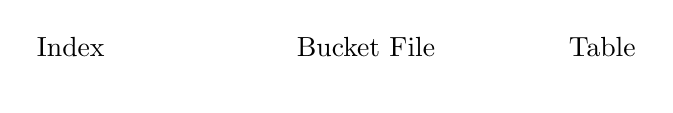
\begin{tikzpicture}
\node at (0,0) [anchor=north] {\scalebox{0.75}{\usebox{\bucketFile}}};
\node at (-3.25,0.25) {\alert{Index}};
\node at (0.5,0.25) {\alert{Bucket File}};
\node at (3.5,0.25) {\alert{Table}};
\end{tikzpicture}
\end{center}
\end{frame}


\begin{frame}{Finding Tuples}
\label{finding_tuple_ids_with_buckets}

Note that the index has no duplicate entries for tuples with the same value. 

To find all tuples within a range $(v_1, v_2)$, we need two pointers. 

\floatstyle{plaintop}
\restylefloat{algorithm}

\begin{center}
\scalebox{0.75}{\begin{minipage}{1.25\textwidth}%
\begin{algorithm}[H]
\begin{algorithmic}
% \caption{retrieving ids of tuples with $a=x$ with secondary index on $a$}
\State \textbf{answer} $\leftarrow \langle \rangle$
\State $p_1 \leftarrow$ first tuple whose key is \underline{at least} $v_1$
\State $p_2 \leftarrow$ first tuple whose key is \underline{greater than} $v_2$ (or \lstinline[style=SQL]{<EOF>})
\State open bucket file at position $p_1$;
\While{$p_1$ is strictly before $p_2$}
    \State append tuple id in $p_1$ to \textbf{answer};
    \State advance $p_1$
\EndWhile
\State \Return \textbf{answer}
\end{algorithmic}
\end{algorithm}
\end{minipage}}
\end{center}
\end{frame}



%
% -----------------------------------------------------------------------
%
\begin{frame}

\textbf{Example:} table $R(a,b,c,d)$;\\
\textbf{primary index} on $R.a$;\\
\textbf{secondary indexes} on $R.b$ and $R.c$.

\vskip2em

\begin{center}
\scalebox{0.75}{\usebox{\whereClauseWithBuckets}}
\end{center}

\end{frame}

%
% -----------------------------------------------------------------------
%
\begin{frame}[fragile]{Complex selections with tuple ids}

The DBMS can solve an arbitrary selection using lists of tuple ids that satisfy each predicate separately.

\begin{columns}[onlytextwidth]
\begin{column}{0.25\textwidth}

\vskip1em
\begin{lstlisting}[style=SQL]
SELECT d
FROM R
WHERE b = 7 AND c = 13;
\end{lstlisting}

\vskip2em

\end{column}

\begin{column}{0.6\textwidth}
\qquad
\scalebox{0.75}{
\begin{tikzpicture}[semithick,align=center,node distance=1cm,every node/.style={inner sep=1,outer sep=1,font=\footnotesize}]
\node (0) at (0,0) {} ; %empty node with ``answer''
\node (1) [below of= 0] {$\pi_{\texttt{d}}$};
\node (2) [below of= 1] {\lstinline[style=SQL]{pointer_lookup}};
\node (3) [below of= 2] {\lstinline[style=SQL]{intersect_id_lists()}};
\node (4) [below left of =3,xshift=-4em,yshift=-0.5em] {\lstinline[style=cmput391]{get_ids(IDX_R_b, 7, 7)}};
\node (5) [below right of =3,xshift=4em,yshift=-0.5em] {\lstinline[style=cmput391]{get_ids(IDX_R_c, 13, 13)}};
\path[->]
    (4) edge (3)
    (3) edge (2)
    (2) edge (1)
    (1) edge (0)
    (5) edge (3);
    
\pause
\node (5) [node distance=3cm,left of=2,color=blue] {\begin{minipage}{2.15cm}\baselineskip=0.75\baselineskip \centering
needed to retrieve attribute 'd'
\end{minipage}};
\draw [color=blue,->] (5) -- (2);
\end{tikzpicture}}
\end{column}
\end{columns}

\vskip2em

\lstinline[style=cmput391]{get_ids(IDX_R_b, b=7)} = $\langle\alert{t_3},\alert{t_4},\alert{t_6}\rangle$

\lstinline[style=cmput391]{get_ids(IDX_R_c, c=13)} = $\langle\alert{t_6},\alert{t_8}\rangle$

\end{frame}

%
% -----------------------------------------------------------------------
%
\begin{frame}

\vskip2em

\begin{columns}[onlytextwidth]
\begin{column}{0.5\textwidth}
\begin{center}
\textbf{Conjunction $\sigma_{c_1 \wedge c_2}(R)$}
\vskip1em
\alert{list intersection}
\vskip1em

\scalebox{0.75}{
\begin{tikzpicture}[semithick,align=center,node distance=1cm,every node/.style={inner sep=1,outer sep=1,font=\footnotesize}]
\node (0) at (0,0) {} ; %empty node with ``answer''
\node (3) [below of= 0] {\lstinline[style=SQL]{intersect_id_lists}};
\node (4) [below left of =3, xshift=-3em,yshift=-0.5em] {\lstinline[style=SQL]{get_ids(IDX_R,}$c_1$\lstinline[style=SQL]{)}};
\node (5) [below right of =3, xshift=3em,yshift=-0.5em] {\lstinline[style=SQL]{get_ids(IDX_R,}$c_2$\lstinline[style=SQL]{)}};
\path[->]
    (4) edge (3)
    (3) edge (0)
    (5) edge (3);
\end{tikzpicture}}
\end{center}
\end{column}
\begin{column}{0.5\textwidth}
\begin{center}
\textbf{Disjunction $\sigma_{c_1 \vee c_2}(R)$}
\vskip1em
\alert{list union}
\vskip1em

\scalebox{0.75}{
\begin{tikzpicture}[semithick,align=center,node distance=1cm,every node/.style={inner sep=1,outer sep=1,font=\footnotesize}]
\node (0) at (0,0) {} ; %empty node with ``answer''
\node (3) [below of= 0] {\lstinline[style=SQL]{union_id_lists}};
\node (4) [below left of =3, xshift=-3em,yshift=-0.5em] {\lstinline[style=SQL]{get_ids(IDX_R,}$c_1$\lstinline[style=SQL]{)}};
\node (5) [below right of =3, xshift=3em,yshift=-0.5em] {\lstinline[style=SQL]{get_ids(IDX_R,}$c_2$\lstinline[style=SQL]{)}};
\path[->]
    (4) edge (3)
    (3) edge (0)
    (5) edge (3);
\end{tikzpicture}}
\end{center}
\end{column}
\end{columns}

\vskip2em

Because tuple ids are \textbf{clustered} in the bucket files, this approach can lead to very fast answers!

\end{frame}


\begin{frame}{I/O cost}

How many blocks are read to find (the identifiers of) all tuples satisfying $v_1 \leq a_i \leq v_2$?

\begin{enumerate}[label=(\arabic*)]
\item number of blocks of the index to find the pointers: $O(h)$, where $h$ is the height of the B+tree

\item number of blocks of the bucket file: $\ceil*{s(R,v_1 \leq a_i \leq v_2)\cdot(\text{\# blocks in bucket file})}$
\end{enumerate}

\vskip1em

The query plan incurs more I/O operations to bring the pointers from the base table, so that the attributes can be read.

\end{frame}


%
% -----------------------------------------------------------------------
%
\begin{frame}

\vskip2em
\begin{columns}[onlytextwidth]
\footnotesize
\begin{column}{0.54\textwidth}
\textbf{Example:} $R(a,b)$; 1 million tuples:\\
- 1000 distinct values of attribute $a$;\\
- 200 distinct values of attribute $b$

\vskip0.5em
Each disk block can hold:\\
- 50 tuples or\\
- 200 key-pointer pairs or\\
- 400 tuple ids
\end{column}
\begin{column}{0.45\textwidth}
\framebox{\begin{minipage}{\textwidth}
file sizes:\\[1em]
- data: 20,000 blocks\\
- B+ tree on $R.a$: \pause \alert{2 levels}\\
- bucket file $R.a$: \pause \alert{2,500 blocks}\\
- B+ tree on $R.b$: \pause \alert{1 level}\\
- bucket file $R.b$: \pause \alert{2,500 blocks}
\end{minipage}}
\end{column}
\end{columns}

\vskip1em

\highlight{I/O cost of $\sigma_{a=k_1 \wedge b=k_2}(R)$:}

\vskip1em

\small
\textbf{Option 1 --} table scan: ~~ $20,000$ 

\textbf{Option 2 --} merging lists:\\

\pause \(3 + 
\pause \ceil*{2,500\cdot s(R,\text{\lstinline[style=SQL]!a!}=k_1)+ 
\pause 2,500 \cdot s(R,\text{\lstinline[style=SQL]!b!}=k_2)} + 
\pause \min \left( s(R,\text{\lstinline[style=SQL]!a!}=k_1) , s(R,\text{\lstinline[style=SQL]!b!}=k_2)  \right) \cdot T(R) \)
\end{frame}


\begin{frame}

\highlight{I/O cost of $\sigma_{a=k_1 \wedge b=k_2}(R)$:}

\vskip1em


\begin{columns}[onlytextwidth]
\begin{column}{0.6\textwidth}
\small
\textbf{Option 3 --} Scan a single index:

\vskip1em

If one predicate has a \emph{much lower} selectivity than the other, the DBMS can read from one of the indexes and evaluate the other predicate after the tuple is retrieved from the database.
\end{column}

\begin{column}{0.4\textwidth}
\begin{center}
\scalebox{0.8}{
\begin{tikzpicture}[semithick,align=center,node distance=0.75cm,every node/.style={inner sep=1,outer sep=1,font=\footnotesize}]
\node (0) at (0,0) {} ; %empty node with ``answer''
\node (1) [below of= 0] {$\sigma_{\texttt{b=}k_2}$};
\node (2) [below of= 1] {\lstinline[style=cmput391]{pointer_lookup}};
\node (3) [below of= 2] {\lstinline[style=cmput391]{get_ids(IDX_on_a, a=}$k_1$)};
\path[->]
    (3) edge (2)
    (2) edge (1)
    (1) edge (0);
\end{tikzpicture}}
\end{center}
\end{column}
\end{columns}

\vskip1em

\small

Ex: Assuming $s(R, \text{\lstinline[style=SQL]!a!}=k_1) \ll s(R,\text{\lstinline[style=SQL]!b!}=k_2)$

The cost would be
\[
\left( 2 +  
\pause \ceil*{2,500 \cdot s(R, {\texttt{a}=k_1}})  +
\pause  \right) + \ceil*{T(R)\cdot s(R,\texttt{a}=k_1)} 
\]
\end{frame}













